
\documentclass[11pt,a4paper]{article}
\usepackage[top=3cm, bottom=2cm, left=2cm, right=2cm]{geometry}
\usepackage[utf8]{inputenc}
% \usepackage[T1]{fontenc}
\usepackage{amsmath, amsfonts, amssymb}
\usepackage{siunitx}
\usepackage[brazil]{babel}
\usepackage{graphicx}
\usepackage[margin=10pt,font={small, it},labelfont=bf, textfont=it]{caption}
\usepackage[dvipsnames, svgnames]{xcolor}
\DeclareCaptionFont{MediumOrchid}{\color[svgnames]{MediumOrchid}}
\usepackage[pdftex]{hyperref}
\usepackage{natbib}
\bibliographystyle{plainnat}
\bibpunct{[}{]}{,}{s}{}{}
\usepackage{color}
\usepackage{footnote}
\usepackage{setspace}
\usepackage{booktabs}
\usepackage{multirow}
\usepackage{subfigure}
\usepackage{fancyhdr}
\usepackage{leading}
\usepackage{indentfirst}
\usepackage{wrapfig}
\usepackage{mdframed}
\usepackage{etoolbox}
\usepackage[version=4]{mhchem}
\usepackage{enumitem}
\usepackage{caption}
\usepackage{titlesec}
\usepackage{tcolorbox}
\usepackage{tikz}
\usepackage{LobsterTwo}
\usepackage[T1]{fontenc}
\usepackage{fontspec}
\usepackage{txfonts}
\AtBeginEnvironment{equation}{\fontsize{13}{16}\selectfont}


\titleformat{\section}{\LobsterTwo\LARGE\color{CarnationPink}}{\thesection.}{1em}{}
\titleformat{\subsection}{\LobsterTwo\LARGE\color{CarnationPink}}{\thesubsection}{1em}{}


\DeclareCaptionLabelFormat{figuras}{\textcolor{DarkTurquoise}{Figura \arabic{figure}}}
\captionsetup[figure]{labelformat=figuras}

\makeatletter
\renewcommand\tagform@[1]{\maketag@@@{\color{CarnationPink}(#1)}}
\makeatother

\renewcommand{\theequation}{Eq. \arabic{equation}}
\renewcommand{\thefigure}{Fig. \arabic{figure}}
\renewcommand{\thesection}{\textcolor{CarnationPink}{\arabic{section}}}

\setlist[itemize]{label=\textcolor{CarnationPink}{$\mathbf{\square}$}}

\setlist[enumerate]{label=\textcolor{CarnationPink}{\arabic*.}, align=left}


\newcounter{exemplo}

\NewDocumentEnvironment{exemplo}{ O{} }{%
\allowbreak
\setlength{\parindent}{0pt}
  \begin{mdframed}[
  leftline=true,
  topline=false,
  rightline=false,
  bottomline=false,
  linewidth=2pt,
  linecolor=CarnationPink,
  frametitlerule=false,
  frametitlefont=\LobsterTwo\large\color{CarnationPink},
  frametitle={\color{CarnationPink}\LobsterTwo\large #1},
  ]
}{%
  \end{mdframed}
}

\setlength{\fboxsep}{5pt}
\setlength{\fboxrule}{1.5pt}
\usepackage{float}
\renewcommand{\thefootnote}{\alph{footnote}}
\usepackage{url}
\hypersetup{
	colorlinks=true,
	linkcolor=DarkTurquoise,
	filecolor=DarkTurquoise,      
	urlcolor=DarkTurquoise,
	citecolor=DarkTurquoise,
	pdftitle={Exercícios}
}
\pagestyle{fancy}
\fancyhf{}
\renewcommand{\headrulewidth}{0pt}
\rfoot{Página \thepage}

\title{\LobsterTwo\Huge{Raphex}}
\author{\LobsterTwo{2023}\nocite{*}}
\date{\LobsterTwo\textit{Dalila Mendonça}}
\begin{document}
	\maketitle

    \begin{enumerate}
        \item Para radiação eletromagnética, o comprimento de onda, λ, pode ser encontrado usando a relação $\lambda$ = c / $\nu$, onde c = 3 x $^108$ m/s é a velocidade da luz e $\nu$ é a frequência eletromagnética.
        
        \item Na mecânica clássica, a energia cinética (KE) é dada por $1/2m\cdot v^2$. Se a massa é 10 kg e a velocidade é 5 m/s, KE = 1/2 (10 kg) $(5 m/s)^2$ = 125 kg $m^22/s^2$ = 125 J.
        
        \item Dose equivalente é a quantidade que representa a medida do dano biológico ao tecido vivo como resultado da exposição à radiação, e a unidade SI de dose equivalente é o sievert (Sv). Tanto o sievert quanto o gray são equivalentes a J/kg, mas diferem um do outro por um fator adimensional (fator de qualidade Q) que explica o efeito biológico do tipo de radiação. Rad e rem são as unidades do sistema CGS para dose absorvida e dose equivalente, respectivamente. O roentgen (R) é uma unidade de exposição à radiação antiga.
        
        \item O principal isótopo de um átomo de hidrogênio consiste em um elétron e um núcleo que contém apenas um próton. Se o átomo é ionizado e perde seu elétron, a única coisa que resta é um próton.
        
        \item Como a energia equivalente de 1 amu é 931 MeV, e a massa total das partículas finais é maior que a das partículas iniciais (0.001281 amu), a reação é endoenergética (endotérmica), ou seja, deve-se aplicar pelo menos 1,19 MeV de energia para a reação ocorra.
        
        \item No decaimento beta menos, um nêutron é convertido em próton, elétron e anti-neutrino.
        
        \item O decaimento do pósitron e a captura de elétrons podem ocorrer quando o núcleo tem um excesso de prótons, portanto esses processos de decaimento competem entre si.
        
        \item O decaimento beta é mediado pela força fraca no Modelo Padrão da física de partículas.
        
        \item A qualidade do feixe é uma especificação da energia de um feixe de radiação. A qualidade do feixe de raios X diagnósticos é definida pela camada semi-redutora (HVL) usando uma geometria de feixe estreito. Irradiadores de raios gama como \ce{^{60}Co} ou \ce{^{137}Cs} são definidos a partir da energia média da radiação gama emitida, e a qualidade do feixe do acelerador linear terapêutico é definida pela porcentagem de dose de profundidade PDP.
        
        \item A probabilidade de produção de raios X bremsstrahlung aumenta com o aumento da energia do elétron incidente. Com o aumento da energia do elétron, a distribuição dos raios-x bremsstrahlung também se torna mais “apontada para frente”, em outras palavras, mais focada na mesma direção que a direção de incidência do elétron sobre o alvo. É por isso que um alvo de transmissão é usado em aceleradores lineares médicos.
        
        \item O feixe que sai de um tubo de raios X superficial será polienergético. A adição de filtração removerá os fótons do feixe, diminuindo a fluência do feixe. Quanto aos fótons que interagem com o filtro, os fótons de baixa energia são preferencialmente absorvidos, resultando em uma energia de feixe média mais alta.
        
        \item A energia máxima de raios X corresponde à tensão de pico do tubo (kVp). Os picos no espectro, indicados como B e C na figura, correspondem às energias de raios X características para o material alvo. A área sob a curva representa o número total de fótons medidos. A energia mínima de raios X é uma função da filtração inerente e adicional do tubo de raios X. Sem filtração, as energias de raios X muito próximas de zero estariam no espectro.
        
            \begin{center}
                \fcolorbox{DarkTurquoise}{white}{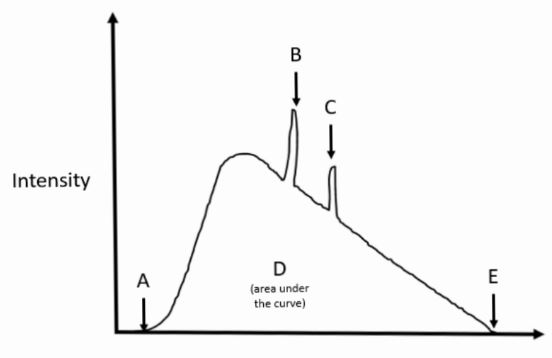
\includegraphics[width=0.4\textwidth]{Imagens/R23_E12.jpg}}
            \end{center}
        
        \item O copo de focalização ``focusing cup'' é carregado negativamente para direcionar os elétrons carregados negativamente para longe do cátodo onde o ``copo'' está localizado e do qual os elétrons são emitidos em direção ao ânodo.
        
        \item As Klystrons amplificam as micro-ondas que são alimentadas no guia de ondas de aceleração, onde fornecem a energia usada para acelerar os elétrons gerados pelo canhão de elétrons.
        
        \item Como o posicionamento correto das partes mecânicas de um linac é extremamente importante para a entrega precisa da radiação, os parâmetros mais críticos do linac são medidos por dois dispositivos calibrados independentes um do outro ``secondary positioning readout devices''. Os dispositivos de leitura secundários são comumente utilizados para confirmar a posição do gantry, colimador, jawns e MLCs do acelerador. Se as leituras das posições primária e secundária discordarem, o linac gerará um intertravamento e interromperá a administração do tratamento.
        
        \item A maioria das lâminas dos MLCs são projetadas com uma extremidade curvada da lâminas para produzir uma penumbra semelhante, independentemente da posição da lâminas. Um projeto alternativo é ter uma extremidade da  lâminas plana, porém o MLC precisará se mover em  arco acompanhando a divergência do feixe.
        
        \item Um linac clínico é um acelerador de elétrons. Assim, tanto para entrega de elétrons quanto para fótons, um canhão de elétrons é usado para injetar elétrons na guia de onda aceleradora. Os elétrons são acelerados para energias de MeV. Se o modo de entrega for o feixe de elétrons, uma folha espalhadora é colocada no caminho do feixe para espalhar o feixe de elétrons de forma que eles possam cobrir o alvo. Se o modo de entrega for feixes de fótons, um alvo é colocado no caminho do feixe estreito de elétrons para que os elétrons interajam e criem fótons via bremsstrahlung. Esses fótons então viajam através de um filtro aplanador (ou não caso seja FFF) para cobrir o alvo com um feixe homogêneo (plano). Na entrega de fótons ou elétrons, uma câmara monitora é usada para medir o output da radiação do linac.
        
        \item Uma guia de ondas preenchida com micro-ondas é usado para acelerar elétrons na faixa de megavoltagem. As guias de onda podem ser usados com ondas estacionárias ou progressivas. Devido à potencial formação de arcos elétricos, a aplicação direta de milhões de elétron-volts entre o cátodo e o ânodo de um tubo de raios X não é normalmente empregada. O campo magnético do ímã de flexão (bending magnet) muda a direção dos elétrons em vez de sua energia. A cavidade buncher é um componente de uma klystron que ajuda a gerar a energia de micro-ondas. (Arcos elétricos são fenômenos que ocorrem quando uma corrente elétrica flui através do ar ou de outro meio isolante. Eles são caracterizados por uma descarga elétrica visível que forma um arco luminoso entre dois pontos de alta tensão. Quando a tensão elétrica em um sistema excede a capacidade de isolamento do ar ou de outro meio dielétrico presente, ocorre uma ruptura na barreira isolante e um arco elétrico é formado. Essa ruptura pode acontecer devido a um curto-circuito, falha na isolação ou por outros motivos.)
        
        \item A distância da fonte de radiação à superfície do paciente (SSD) é medida pelo indicador óptico de distância (ODI). A SAD é a distância da fonte ao isocentro da máquina e é fixo para uma determinada máquina. Uma ponteira frontal pode ser usada para identificar a localização física do isocentro. O tamanho do campo luminoso pode ser medido usando papel quadriculado, e os campos luminosos e radiativos devem ser coincidentes. Essa coincidência pode ser verificada por meio de um filme de raio-x.
        
        \item Uma mesa com seis graus de liberdade pode se mover nas direções de translação lateral, vertical e longitudinal, bem como nas rotações de inclinação pitch, rotação roll e rotação yaw. Uma roll é uma rotação ao longo plano axial do paciente, uma pitch é uma rotação ao longo do plano sagital do paciente e uma rotação guinada yall - também conhecida como ângulo de mesa - é uma rotação ao longo do plano coronal do paciente, conforme ilustrado no diagrama.
        
        \begin{center}
            \fcolorbox{DarkTurquoise}{white}{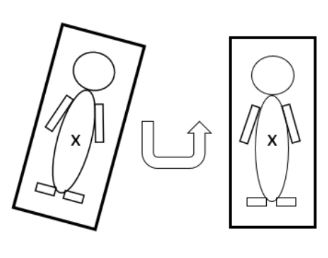
\includegraphics[width=0.4\textwidth]{Imagens/R23_E20.JPG}}
        \end{center}

        \item Como o coeficiente de atenuação do feixe é inversamente proporcional à energia do feixe, a camada semi-redutora  $[HVL = (ln 2) / \mu]$ aumenta pois a energia média do feixe transmitido aumenta, ou seja, o feixe torna-se cada vez mais “duro” à medida que a espessura do absorvedor aumenta e portanto a segunda HVL é maior porque o $\mu$ se torna menor.
        
        \item O nome da interação entre um fóton e um elétron atômico onde o fóton transfere toda a sua energia para o elétron e esse elétron é ejetado do átomo é ``efeito fotoelétrico''. No caso de uma ionização da camada interna, além da ejeção do fotoelétron, também haverá emissão subsequente de raios-x característicos ou elétrons Auger à medida que os elétrons orbitais com  maior energia caem para preencher a camada interna. O espalhamento Compton é uma interação entre um fóton e um “elétron aproximadamente livre”, ou seja, um elétron com energia de ligação desprezível. Após uma interação Compton, o fóton espalhado e o elétron compartilham a energia que foi inicialmente transportada pelo fóton incidente.
        
        \item Em uma interação de espalhamento Compton entre um fóton e um elétron, o fóton espalhado sempre reterá pelo menos 256 keV de energia. Nesta situação, o fóton é retroespalhado e o elétron é projetado na direção de propagação do fóton incidente.
        
        \item Em uma interação de produção de pares, um fóton interage com o campo de um núcleo. Como resultado da interação, o fóton desaparece e um par elétron/pósitron é criado. A energia total da massa de repouso de um elétron e um pósitron é 1,022 MeV. Para respeitar a conservação de energia e momento, essa interação não pode ocorrer a menos que o fóton incidente tenha uma energia de pelo menos 1,022 MeV.
        
        \item Partículas diretamente ionizantes são partículas carregadas que, ao viajarem através de um meio, podem ionizar os átomos dentro do meio por meio de interações mediadas através da força eletromagnética existente em partículas carregadas. Partículas indiretamente ionizantes não possuem carga. Eles precisam ter uma interação com o meio que cria uma partícula carregada, que posteriormente deposita energia por meio de interações de força eletromagnética.
        
        \item A geometria de feixe estreito mede apenas a atenuação do feixe primário. Quaisquer fótons secundários ou dispersos não podem ser incluídos na medição. Diz-se que uma medição de atenuação que inclui fótons primários, secundários e dispersos é realizada sob condições de “feixe largo”.
        
        \item A unidade Hounsfield é calculada por: $HU = [(\mu_{meio} - \mu_{agua})/\mu_{agua}] \times 1000$; portanto um meio com $HU = 1000$ tem $\mu_{meio} = 2\mu_{agua}$.

        \item A lei do inverso do quadrado afirma que conforme você aumenta a distância, r, de uma fonte pontual de radiação, a intensidade da radiação diminui em $1/r^2$.

        \item Exposição, KERMA e TERMA são todos definidos para partículas não carregadas, mas não para partículas carregadas. A dose é definida para partículas carregadas e não carregadas. CEMA (Converted Energy per unit MAss - ); TERMA (Total Energy Release per unit MAss); KERMA (Kinetic Energy Release per unit MAss)
        
        \item KERMA é definido como a quantidade de energia transferida de partículas não carregadas incidentes para partículas carregadas em um meio. TERMA é a energia total transferida das partículas não carregadas incidentes para todas as partículas (fótons e elétrons) no meio. Dose é a energia absorvida em uma unidade de massa, exposição é a quantidade de carga liberada no ar e fluência é o número de partículas por unidade de área. CEMA Descreve a transferência de energia de partículas carregadas primárias para partículas carregadas secundárias (raios $\delta$);

        \item O valor esperado do número de partículas que atingem uma esfera finita em torno de um ponto é a definição de fluência. A fluência de energia é semelhante, exceto que corresponde ao valor esperado da energia total transportada por todas as partículas que atingem uma esfera finita em torno de um ponto. O fluxo e o fluxo de energia são a taxa de variação no tempo da fluência e da fluência de energia, respectivamente. A energia radiante é definida apenas como a soma da energia das partículas que foram emitidas, transferidas ou recebidas.

        \item Os diodos são normalmente usados sem tensão de polarização. Um diodo mede um sinal muito forte em relação ao ar (utilizado na cavidade de uma câmara de ionização para medir a dose) porque a densidade do silício é aproximadamente 1.900 vezes a do ar, e a energia necessária para criar um par elétron/buraco no silício é de 3,5 eV, aproximadamente 10 vezes menos que a energia necessária no ar ($\sim$ 33,97 eV) . Os diodos são dosímetros relativos e têm uma dependência direcional maior do que as câmaras de ionização, no entanto, esses fatores não contribuem para as razões pelas quais os diodos mediriam sinais maiores do que as câmaras de ionização para a mesma dose de radiação e mesmo tamanho do detector. 

        \item \textcolor{DarkTurquoise}{\textbf{Em relação a uma câmara Farmer de 0,6 cc, uma câmara de 0,03 cc terá melhor resolução espacial e mais ruído.}} Uma câmara de 0,03 cc é muito menor que uma câmara Farmer e, portanto, terá resolução espacial melhorada, o que resultará em um desempenho superior para medições em campos pequenos. No entanto, esta câmara também experimentará mais ruído nas medidas, e é por isso que, para uma medição de saída em um campo de 10 cm x 10 cm, a câmara Farmer seria uma opção melhor. \textcolor{MediumOrchid}{Porque a câmara de 0.03 cc possui mais ruído nas medidas?}

        \item Na faixa de energia de megavoltagem, o espalhamento Compton é a interação predominante para os fótons. Portanto, para imitar o tecido, o material do phantom deve corresponder à seção de choque do Compton para o tecido, o que ocorre se a densidade de elétrons for compatível.

        \item Fótons com comprimentos de onda na faixa da luz visível são liberados quando um TLD é aquecido após ser exposto à radiação ionizante. A intensidade da luz emitida é tipicamente medida por um tubo fotomultiplicador.

        \item O adendo do AAPM Task Group 51 observa que a recombinação iônica contabilizada no fator de recombinação $P_{ion}$ é aumentada para feixes com maior dose por pulso, como ocorre nos feixes FFF.

        \item Ao considerar detectores para medida da dose na superfície do paciente: Os detectores MOSFET de baixa voltagem podem ser usados na clínica para medir a dose de radiação \textit{in vivo} para qualquer modalidade (fótons, elétrons, hadrons\dots) e eles possuem espessura insignificante. As câmaras de ionização usam alta voltagem, o que seria inseguro para o paciente. Medidores de levantamento (Geiger) detectam radiação, mas são grandes e não podem fornecer informações de dosimetria in vivo. O filme radiocrômico precisa ser cuidadosamente manuseado e calibrado, tornando-o muito difícil de usar para dosimetria in vivo.

        \item Uma câmara de ionização de ar livre mede a quantidade de exposição, que é uma medida da carga elétrica produzida quando um feixe de fótons interage com uma massa conhecida de ar. Por definição, a câmara deve conter ar e, portanto, não seria mantida no vácuo. Não há exigência de que o feixe de fótons incidente seja monoenergético, embora por razões práticas relacionadas à atenuação e espalhamento e a consequente faixa de elétrons secundários, uma câmara de ionização ao ar livre não possa medir energias de fótons maiores que aproximadamente 3 MeV. Uma câmara de ionização de ar livre usa um campo elétrico uniforme em sua região de coleta para coletar e medir toda a carga liberada. Um tubo de raios X é frequentemente submerso em um banho de óleo para dissipação de calor, mas uma câmara de ionização ao ar livre não esquenta como um tubo de raios X e não é colocada em um banho de óleo.

        \item O eletrodo de proteção ``guard electrode'' de uma câmara de ionização é usado para isolar a câmara de ionização para que as cargas criadas no volume ativo não escapem. Como resultado, a colocação do eletrodo de guarda define o limite do volume ativo.

        \item Câmaras de ionização, diodos, contadores proporcionais, contadores Geiger-Muller são lidos instantaneamente no momento da irradiação usando um eletrômetro ou dispositivo de leitura. Os OSLDs são coletados após serem irradiados e colocados em um dispositivo específico que lê a quantidade de luz visível liberada quando o cristal é estimulado com uma luz de laser. Essa quantidade de luz visível emitida pode estar relacionada à dose absorvida pelo OSLD.

        \item Em um tratamento de neuroeixo, para combinar a divergência dos campos cranianos com a divergência dos campos da coluna, os dois ângulos $\theta_{coll}$ e $\theta_{couch}$ são determinados a partir das seguintes relações: $$\theta_{coll} = \arctan \left(\frac{1/2 L_1}{100}\right)$$  $$\theta_{couch} = \arctan \left(\frac{1/2 L_2}{100}\right)$$ onde $L_1$ é o comprimento do campo da coluna e $L_2$ é o comprimento do campo cranial. \textcolor{MediumOrchid}{Revisar essa relação para determinar se é o campo na SAD ou SSD ou SPD}

        \item Se dois campos posteriores da coluna forem usados para cobrir o comprimento da coluna vertebral, como em um tratamento de neuroeixo, esses campos devem se cruzar em um ponto localizado anteriormente à medula espinhal para evitar regiões de alta dose dentro da medula. Isso é verdade mesmo quando é utilizada uma técnica de feathering (diluição, difusão.. faço a menor ideia do nome disso em pt-Br).
        
        \item A largura da penumbra geométrica em qualquer profundidade da superfície de um paciente é dada por$$ P_d = s (SSD + d – SDD) / SDD$$ onde $s$ é a dimensão da fonte, $SSD$ é a distância da fonte à superfície e $SDD$ é a distância fonte-diafragma (colimador)

        \item A relação tecido-máximo, TMR, é independente da distância fonte-superfície, SSD e, portanto, independente da queda da fluência com inverso do quadrado da distância até a fonte.

        \item Para feixes de fótons isocêntricos, a fórmula de cálculo de MU é: MU = (dose por fração / número de campos) / [saída de referência x Sc(CS) x Sp(FS) x TMR(d, FS)], onde CS é o colimador configuração e FS é o tamanho do campo irradiado na profundidade d. Como não há bloqueio, o FS no isocentro é equivalente ao CS. O CS e FS a usar para este campo assimétrico podem ser encontrados usando a regra de área/parâmetro: 4 x (área) / (perímetro) = 4 x (6)(12) / [2 x (6 + 12)] = 8, então você procuraria Sc, Sp e TMR para um campo de 8 cm x 8 cm. MU = (400 / 2) / (1,0 x 0,987 x 0,990 x 0,871) = 235.
        
        \item Se os MLCs fossem utilizados para adicionar bloqueio nos campos de tratamento, mas nenhum outro parâmetro fosse alterado o Sc permaneceria o mesmo e Sp diminuiria. Sc depende da posição dos jaws do colimador e, portanto, não mudaria. Sp depende do tamanho efetivo do campo bloqueado e diminui conforme o tamanho do campo diminui.

        \item \textcolor{DarkTurquoise}{\textbf{Em relação à dose de superfície de raios-x MV:}}
            \begin{itemize}[label=\textcolor{CarnationPink}{$\star$}]
                \item os sistemas de planejamento de tratamento geralmente não calculam com precisão a dose de superfície;
                \item os elétrons produzidos no cabeçote do linac são um grande componente da dose de superfície;
                \item a dose de superfície de um feixe de 15 MV é menor do que a de um feixe de 6 MV;
                \item a dose de superfície aumenta com o tamanho do campo;
                \item Um feixe sem filtro aplanador (FFF) terá uma dose superficial mais alta do que um feixe com filtro aplanador com o mesmo potencial de ionização para a maioria dos tamanhos de campo. \textcolor{MediumOrchid}{O que é o potencial de ionização e porque eles sendo o mesmo para o feixe FFF e o feixe FF a dose na superfície será a mesma?}
            \end{itemize}

        \item \textcolor{DarkTurquoise}{\textbf{A PDP a 10 cm de um feixe FFF de 6 MV é aproximadamente 3\% menor em comparação com um feixe FF de 6 MV.}} O filtro aplanador remove fótons de baixa energia do feixe causando seu endurecimento, ou seja, aumenta a energia média do feixe plano em relação a um feixe que não utiliza um filtro aplanador (FFF). O resultado do feixe plano mais endurecido é a diminuição da atenuação com a profundidade e um aumento na PDP quando comparada ao feixe FFF com mesma energia nominal.

        \item À medida que o SSD aumenta, o PDD aumenta devido à diferença no componente quadrado inverso do PDD. O fator de correção, conhecido como fator Mayneord, que converte curvas PDD de um SSD para outro, é: $$F = \left(\frac{SSD_2 + d_m}{SSD_1 + d_m}\right)^2 \cdot \left(\frac{SSD_1 + d}{SSD_2 + d}\right)^2$$ 

        \item A densidade eletrônica do pulmão é apenas aproximadamente 30\% da densidade da água, resultando em uma menor absorção e um efeito de build-down (desacumulo? hehe) para feixes de MV. Todos os outros locais do corpo são compostos de tecidos com densidades de elétrons muito mais próximas da água de modo que as correções de heterogeneidade causem menos efeito no número de MU quando comparado ao pulmão.

        \item A TMR para fótons de 15 MV muda em aproximadamente 2,5\% por cm. Como a profundidade é maior, a dose entregue será menor do que a calculada. Caso um tratamento com geometria de box com os campos com o mesmo peso na técnica isocêntrica; se um dos campos tiver com uma profundidade 3cm maior que a planejada a mudança na dose do isocentro é, portanto, (–2,5\%/cm x 3 cm) / 4, ou aproximadamente –2\%. \textcolor{MediumOrchid}{Quais são os valores aproximados para as mudanças em feixes de 6MV e 10 MV?}

        \item O flash de pele (skin flash) é comumente usado no planejamento 3D de alvos próximos à pele, como mama ou crânio total (whole brain), para garantir que todo o alvo permaneça dentro do campo na presença de incertezas de setup, mudanças na anatomia ao longo do tempo ou, no caso de tratamentos de mama, compensar o movimento respiratório. Fechar o colimador na superfície da pele leva ao risco de subdosagem, enquanto abrir o colimador apresenta pouco ou nenhum risco de exposição de tecido adicional.

        \item \textcolor{DarkTurquoise}{\textbf{O ângulo do filtro é definido como o ângulo formado entre a linha perpendicular ao eixo central e uma linha de isodose do campo filtrado em uma profundidade específica.}} O ângulo do filtro é o ângulo da linha de isodose em relação à posição da mesma linha de isodose sem o filtro em uma profundidade que tipicamente é de 10 cm.

        \item À medida que a energia do fóton de megavoltagem aumenta, a profundidade de $D_{max}$ aumenta porque a energia média dos elétrons secundários aumenta. O valor da porcentagem de dose na profundidade (PDP) a 10 cm aumenta à medida que há menos atenuação para energias mais altas.

        \item A configuração do colimador é definida em 100 cm (isocentro). Para configuração de 100 SAD, o tamanho do campo (25cm x 25 cm) está na profundidade do tumor (5 cm). Para uma configuração de SSD igual a 120 cm, o tamanho de campo necessário (a 100 cm) pode ser calculado por 25 cm x (100/125) = 20 cm.

        \item Monte Carlo continua sendo o algoritmo de cálculo de dose mais preciso principalmente se tratando da presença de heterogeneidade, seguido pelos algoritmos de convolução/superposição, algoritmos de convolução de pencil beam e, finalmente, algoritmos de TAR equivalente.

        \item A planura do feixe está relacionada com as doses máximas e mínimas em um plano dentro de 80\% do campo que é dada por $$Planura = \left(\frac{D_{max} - D_{mim}}{D_{max} + D_{mim}}\right)\times 100$$ A simetria do feixe é a diferença percentual na dose entre dois pontos em lados opostos do eixo central (CAX). A razão fora do eixo (OAR - razão off-axis) é a razão da dose em um ponto distante do CAX (eixo central) para aquele no CAX. A PDP e a ração máxima de tecido (TMR) são medidas distalmente ao longo do CAX, perpendicularmente ao plano do perfil do feixe.

        \item \textcolor{DarkTurquoise}{\textbf{A fonte principal de dose de fótons fora do campo de tratamento para o paciente é devido ao espalhamento do paciente nas proximidades da borda do campo, mas depois muda para a fuga do cabeçote a aproximadamente 20 cm da borda do campo.}} Conforme especificado no relatório do AAPM Task Group 158, próximo à borda do campo, a dose fora do campo ocorre principalmente devido ao espalhamento no paciente, que então muda para a radiação de fuga do cabeçote do acelerador à medida que a distância do alvo aumenta. 

        \item Como regra geral, a profundidade de tratamento de um feixe de elétrons MeV, $R_{90}$ em centímetros, pode ser estimada como a energia do elétron em MeV dividida por 3.2. Para uma profundidade de 3.75 cm O uso de uma energia de elétron maior que 12 MeV forneceria mais dose ao pulmão e aos tecidos localizados distalmente ao alvo sem fornecer cobertura de alvo adicional.

        \item O alcance de elétrons de 12 MeV em água/tecido mole é de aproximadamente 6 cm, dado por energia (MeV) / 2. A atenuação por uma dada espessura z de uma heterogeneidade é equivalente à atenuação (z x CET) da água, onde “CET ” significa “coeficiente de espessura equivalente”. O CET é a razão entre a densidade eletrônica do material e a densidade eletrônica da água, então um CET de 1.5 implica que o osso tem 1.5 vezes a densidade eletrônica da água. Depois de percorrer 3 cm de tecido mole, o feixe tem 3 cm de comprimento de caminho equivalente de tecido mole restante. Uma atenuação de 2 cm no osso com CET de 1,5 é equivalente à atenuação de 3 cm na água. Portanto, o alcance geométrico deste feixe de elétrons de 12 MeV neste phantom será de 5 cm (3 cm em tecido mole e 2 cm em osso).
        
        \item Em relação a um feixe direto de elétrons, o aumento da obliquidade em um campo faz com que a profundidade da dos0e máxima se mova em direção à superfície do paciente, e a curva de dose na profundidade cai mais rapidamente após atingir o valor máximo à medida que a obliquidade aumenta. O impacto normalmente se torna significativo para ângulos de 45 graus ou mais. Nos cálculos manuais, o impacto é contabilizado com um fator de obliquidade que depende do ângulo e da profundidade dentro do paciente.

        \item Dentre a folha espalhadora, os jaws colimadores, os blocos para elétrons e o tecido do paciente, o que menos contribui para a contaminação do feixe com raios-x é o tecido do paciente. A maior parte da contaminação por raios X em um feixe de elétrons de tratamento resulta de interações de bremsstrahlung com materiais de alto número atômico na cabeça do linac (folhas espalhadoras, jaws do colimador, etc.) e o bloco de colimação de elétrons (cutout). Embora possa haver alguns raios-x criados a partir de interações dentro do paciente, o número é muito menor do que o proveniente da cabeça do linac.

        \item Para feixes de elétrons, as unidades monitoras são calculadas usando MU = (dose de prescrição por fração) / (linha de isodose de prescrição/100\%) / (saída de referência x cone medido/fator de cutout). Para este caso, MU = (400 / 0,85) / (1,0 x 1,009) = 466.

        \item Se um tratamento de elétrons de 9 MeV está planejado para uma SSD de 100 cm com um bolus de 1.0 cm dando uma distância fonte-bolus de 99 cm. Dado uma SSD efetiva de 87 cm, se o paciente for tratado com uma distância fonte-bolus de 100 cm, o paciente estará 1 cm mais distante do que o esperado durante a administração da dose e, portanto, receberá uma dose menor do que o planejado. A SSD effetiva é usada para correção de feixe de elétrons com o IQD ($1/r^2$). Assim, se a SSD efetiva de 87 cm corresponder a uma distância do isocentro de 100 cm, aumentar a distância do paciente em 1 cm corresponderá a uma alteração no output de $(87 cm / 88 cm)^2 = 0.98$, mostrando uma diminuição de 2\% na dose entregue.

        \item Para energias de fótons acima de 10 MeV, as interações fotonucleares entre o feixe de fótons de alta energia e os componentes do cabeçote do gantry do acelerador liberarão nêutrons. Os nêutrons são partículas de alto LET que podem danificar componentes eletrônicos, podendo causar falha funcional dos dispositivos implantados.

        \item De acordo com o AAPM Task Group 203, o intervalo de doses recebido no marcapasso de 2 Gy até 5 Gy é classificado como “risco médio” para pacientes que não dependem de marcapasso e estão sendo tratados com feixes de fótons de 6 MV. Qualquer tratamento com energias de fótons superiores a 10 MV é considerado de alto risco devido à presença de contaminação por nêutrons. Se um paciente não for dependente de marca-passo, doses menores que 2 Gy são consideradas de baixo risco. Se um paciente for dependente de marca-passo, qualquer dose inferior a 5 Gy é considerada de médio risco.

        \item De acordo com o relatório do AAPM Task Group 142, a coincidência de coordenadas de imagem e tratamento para um único ângulo do gantry precisa ser verificada diariamente e deve estar dentro de $\leq$ 2 mm para uma máquina que não realiza tratamentos de SRS/SBRT e dentro de $\leq$ 1 mm para uma máquina que realiza tratamentos de SRS/SBRT . A coincidência de coordenadas de imagem e tratamento em 4 ângulos cardeais precisa ser verificada mensalmente.

        \item \textcolor{DarkTurquoise}{\textbf{De acordo com o relatório do AAPM Task Group 142 - e enfatizado novamente na AAPM Medical Physics Practice Guideline 8a sobre testes de desempenho do acelerador linear - o output do linac precisa ser verificado na água de acordo com o AAPM Task Group 51 anualmente.}} Segundo o guideline 8a: \textcolor{MediumOrchid}{\textbf{Depois que os feixes são calibrados com base no TG51, os sistemas de medição secundário (mensal, se aplicável) e terciário (diário) devem ser irradiados para estabelecer ou confirmar as leituras de output do baseline que estão vinculadas à calibração primária (consulte a seção 8.A. deste relatório). O QMP pode usar um sistema de medição secundário (ou seja, à base de água sólida) para verificações mensais de output ou usar um sistema à base de água como feito para calibração anual. O QMP deve decidir sobre os detalhes dos sistemas de medição secundários e terciários; seu atributo fundamental deve ser a reprodutibilidade.}}
        
        \item \textcolor{DarkTurquoise}{\textbf{De acordo com o relatório AAPM Task Group 142, a constância do perfil do feixe (simetria e planura) precisa ser verificada pelo menos mensalmente. Diariamente é necessário ser realizado apenas a constância do output nos testes dosimétricos. Caso o perfil do feixe seja avaliado diariamente (com equipamentos terciários como o daily QA ou QuickCheck) a tolerância é de 2\% do baseline. Nas medidas mensais a tolerância é de 1\% segundo o TG142  (mensal e anual) e de 2\% segundo o Guideline tanto para o mensal quanto para o anual, onde é comparado com o TPS.}}
        
        \item O desalinhamento mecânico dos jaws colimadores afetaria os testes de starshots do colimador, a coincidencia do campo radiativo do campo luminoso, o teste Winston-Lutz baseado no jaw e a definição da borda do campo no teste de radiation beam steering
        
        \item O Grupo de Tarefas 201 da AAPM aborda o gerenciamento de qualidade da transferência de dados de terapia de feixe externo. O sistema de simulação (SS - simulation system) refere-se à aquisição de dados de imagem (potencialmente de múltiplas modalidades) utilizados para o planejamento do tratamento. O sistema de planejamento de tratamento (TPS - treatment planning system) é utilizado para importação/exportação de imagens, contorno e cálculo de dose. O sistema de gerenciamento de tratamento (TMS - treatment management system), também conhecido como sistema de record and verify, armazena e troca dados do TPS com o linac ou outros dispositivos de entrega de radiação, conhecidos como sistema de entrega de tratamento (TDS - treatment delivery system).

        \item De acordo com o AAPM TG-201, o sistema de gerenciamento de tratamento (TMS) contém informações do paciente como um registro médico eletrônico. No entanto, o R\&V também importa e exporta informações para a máquina de tratamento. Portanto, informações demográficas do paciente, agendamento, bem como parâmetros do plano de tratamento e imagens adquiridas são armazenadas. Embora a scan de planejamento possa estar no sistema de gerenciamento de tratamento para alinhamento com as imagens de tratamento adquiridas, os estudos de imagem secundários usados para delinear o alvo estariam no sistema de planejamento de tratamento e não no TMS.

        \item O aprendizado de máquina (Machine learning) é um ramo da inteligência artificial em que os programas de computador recebem um conjunto de dados de treinamento e, a partir desses dados, podem fazer inferências e previsões, sem que o usuário programe explicitamente o algoritmo para fazê-lo. O algoritmo também pode melhorar com o aumento da “experiência”, em outras palavras, a exposição a conjuntos de dados maiores e mais variados. O aprendizado de máquina é usado em muitos aspectos da vida diária, incluindo filtragem de e-mail, reconhecimento de fala, bem como aplicações específicas em oncologia de radiação, como segmentação de imagens.
        
        \item O tipo de detector que utiliza as tensões na região marcada pelo “x” no gráfico abaixo, aproximadamente 1000 a 1400 V é o contador Geiger-Muller. O contador Geiger-Mueller utiliza uma tensão de alta polarização para gerar um sinal uniforme para a radiação recebida. Voltagem adicional aplicada além da região Geiger-Mueller resultaria em uma descarga contínua do detector. O platô na área de baixa tensão é a zona onde operam as câmaras de ionização. A próxima zona à direita, onde há um aumento proporcional da carga coletada com o aumento da tensão aplicada, é a zona onde operam os contadores proporcionais.
        
        \begin{center}
            \fcolorbox{DarkTurquoise}{white}{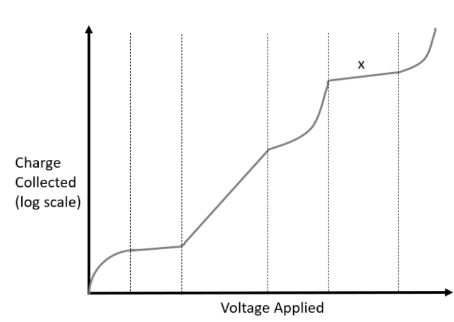
\includegraphics[width=0.4\textwidth]{Imagens/R23_E74.JPG}}
        \end{center}

        \item Em um feixe de fótons, a contaminação por nêutrons aumenta rapidamente à medida que a energia do feixe aumenta de 10 para 20 MV. Os raios X de 6 MV estão abaixo do limiar de energia para interações fotonucleares. Um arranjo de labirinto na sala do acelerador pode reduzir drasticamente o requisito de blindagem para a porta. Com um design de labirinto adequado, a porta é exposta principalmente à multiplas radiação espalhada de intensidade e energia muito reduzidas. Em geral, um labirinto mais longo ($>$5 m) também pode reduzir a fluência de nêutrons na porta. Por outro lado, um labirinto na entrada, será necessária uma porta pesada para fornecer uma blindagem equivalente à parede.

        \item \textcolor{DarkTurquoise}{\textbf{O NCRP recomenda que qualquer pessoa que tenha uma chance razoável de receber pelo menos 10\% do limite de dose regulamentar seja monitorado. O tipo de monitor usado dependerá do tipo de radiação a que a pessoa está exposta. Em oncologia de radiação, o dosímetro é normalmente usado no tronco do corpo com um dosímetro de anel usado na mão (extremidade) ao manusear fontes radioativas.}}

        \item \textcolor{DarkTurquoise}{\textbf{Das seguintes circunstâncias: Implante de próstata guiado por ultrassom com fontes de 125I; Implante de próstata guiado por ultrassom com fontes de 103Pd; Radioterapia intraoperatória de alta taxa de dose; Procedimento de radiologia intervencionista guiado por fluoroscopia e Procedimento de implante LDR de 137Cs. Um avental de chumbo seria mais útil para reduzir a dose recebida em um médico que realiza um procedimento de radiologia intervencionista guiado por fluoroscopia. A energia de emissão de 137Cs (662 keV) é muito alta para ser atenuada por um avental de chumbo. A dose de corpo inteiro para o médico dos isótopos 125I e 103Pd é muito baixa, e um avental de chumbo pode retardar o procedimento e resultar em dor nas costas. Na radioterapia intraoperatória HDR, todos saem da sala de tratamento enquanto a radiação está sendo aplicada, portanto, o avental é desnecessário. Na fluoroscopia, a taxa de dose pode ser significativa e as energias típicas de raios X são baixas o suficiente para que o avental forneça proteção significativa.}}

        \item O fator de uso para fuga é unitário (U = 1), pois a radiação de fuga está presente sempre que a máquina é operada.

        \item O modelo de dano (curva) de radiação que é usado atualmente para estimar o risco devido a exposição à radiação e para estabelecer padrões de proteção radiológica e monitoramento de pessoal é o modelo B apresentado na figura abaixo. Os padrões atuais para estabelecer proteção contra radiação utilizam o modelo linear sem limiar de dose (LNT - linear no-threshold).
        
        \begin{center}
            \fcolorbox{DarkTurquoise}{white}{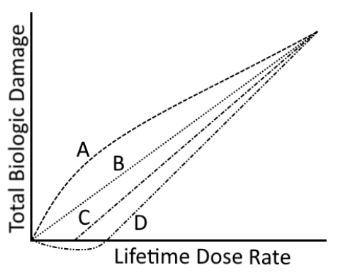
\includegraphics[width=0.4\textwidth]{Imagens/R23_E79.JPG}}
        \end{center}

        \item \textcolor{DarkTurquoise}{\textbf{A profundidade de penetração de um feixe de ultrassom é inversamente proporcional à frequência do transdutor. A regra geral é que um feixe de ultrassom atenua em 0.5 (dB/cm)/MHz. Ondas de ultrassom de frequência mais alta podem detectar objetos menores na direção do feixe. Escolher a frequência de ultrassom apropriada para uma determinada aplicação é um compromisso entre a profundidade de penetração e a resolução espacial.}}

        \item O núcleo dos átomos de hidrogênio tem um spin diferente de zero que é necessário para um átomo produzir um sinal quando submetido a um sinal de radiofrequência enquanto estiver dentro de um campo magnético. Devido à sua alta sensibilidade e alta concentração no corpo humano, os átomos de hidrogênio são a principal fonte de sinal na ressonância magnética.

        \item

        \item

        \item

        \item

        \item

        \item
        
        \item

        \item

        \item

        \item

        \item

        \item

        \item

        \item
        
        \item
        
        \item
        
        \item
        
        \item
        
        \item
        
        \item

        \item

        \item

        \item

        \item

        \item
        
        \item

        \item

        \item
            
        \item

        \item

        \item

        \item

        \item

        \item

        \item

        \item

        \item

        \item

        \item

        \item

        \item

        \item

        \item

        \item
            
        \item
    
        \item
   
        \item
    
        \item
    
        \item
    
        \item
    
        \item
    
        \item
    
        \item
    
        \item
    
        \item
    
        \item
    
        \item
    
        \item
    
        \item
    
        \item
    
    \end{enumerate}


\end{document}